\documentclass[12pt]{article}

% Any percent sign marks a comment to the end of the line

% Every latex document starts with a documentclass declaration like this
% The option dvips allows for graphics, 12pt is the font size, and article
%   is the style




% array/table
\usepackage{array}
\usepackage{multirow}

% figure
\usepackage[pdftex]{graphicx}
\usepackage{epsfig}
\usepackage[hang]{subfigure}
\usepackage[small,bf]{caption}
\usepackage{amsmath}
\usepackage{enumitem}
\usepackage{tabularx}
\usepackage{ctable}


\usepackage{authblk}
\renewcommand\Authands{ and }

%clickable ref
\usepackage[backref,pagebackref,naturalnames=true]{hyperref}



\setlength{\oddsidemargin}{0.25in}
\setlength{\textwidth}{6.5in}
\setlength{\topmargin}{0in}
\setlength{\textheight}{8.5in}



%----------------------------------------------------------------------------------------
%        DOCUMENT INFORMATION
%----------------------------------------------------------------------------------------

\title{}


\author[1]{B. Mouginot  \thanks{\href{mailto:mouginot@wisc.edu}{mouginot@wisc.edu}}}
\author[1]{P.P.H. Wilson\thanks{\href{mailto:paul.wilson@wisc.edu}{paul.wilson@wisc.edu}}}
\author[1]{R. Carlsen} 
\author[1]{A. Opotowsky} 
\affil[1]{University of Wisconsin--Madison, Department of Engineering Physics, CNERG group}


\date{\today}

\setlength{\parindent}{0em}
\setlength{\parskip}{0.7em}

\begin{document}
\maketitle

\section{Intro/specification}

This memo presents the modeling results of cases 1.1 to 1.3 of the EG29
scenario, induced by the use of a plutonium equivalent model for the fuel
fabrication. Case 1 of the EG29 calculation involves the modeling of a single
MOX-PWR at steady-state (see figure \ref{fig:puflow}).

\begin{figure}[h!]
  \centering
  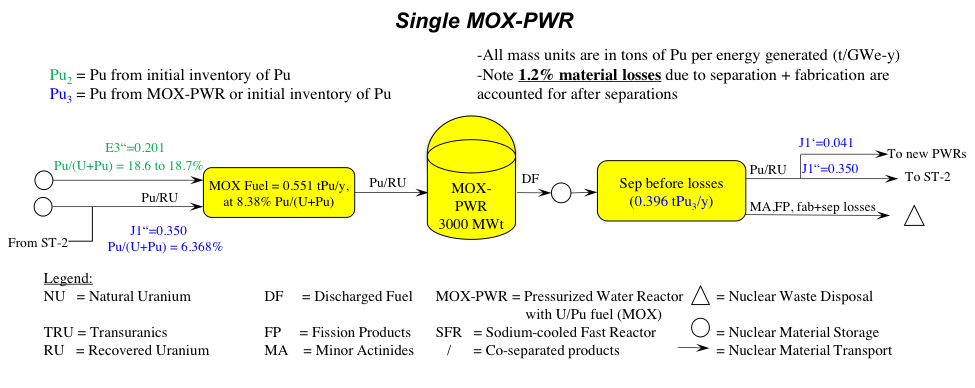
\includegraphics[width=1\textwidth]  {img/puflow}
  \caption{Schematic of Pu mass flow for Case 1.x}
  \label{fig:puflow}
\end{figure}

Case 1 is subdivided into three sub-cases corresponding to calculations of
increasing fidelity: 
\begin{itemize}
  \item	1: without isotopic composition, 
  \item 2: with isotopic composition and no decay,
  \item 3: with isotopic composition and decay.
\end{itemize}


\section{Fix mixing ratio vs Pu-equivalent theory}

The first part of this memo is dedicated to the comparison between fixed ratio
mix and Pu-equivalent theory for the fuel fabrication process.

Two variations on fuel-building were calculated for each sub-case (1.1 to 1.3).
The first calculation used a standard mixing fab (in Cyclus, the
''cycamore::mixer''). This mixed the E3” and the J1” streams using a constant mixing
ratio to build the MOX fuel for the PWR, labeled “M”. The second calculation
used plutonium equivalent theory to determine the mixing fraction of each stream
to build the MOX fuel, labeled “W”.

\begin{figure}[h!]
  \centering
  \subfigure[J1'' stream plutonium flow\label{fig:J1s}] 
    {\epsfig{figure=img/C_1_x_J1s_pu_contribution,width=0.48\textwidth}}
  \subfigure[E3'' stream plutonium flow\label{fig:e3s}] 
    {\epsfig{figure=img/C_1_x_E3s_pu_contribution,width=0.48\textwidth}}
  \caption{Evolution of the plutonium content in the J1'' and  E3'' stream\label{fig:MW_flow} }
\end{figure}

The difference on J1'' and E3'' between all 6 calculations can be observed on
Figure \ref{fig:MW_flow}. First one should only consider in this study the time
after 15 and 75y, as the calculation need almost 12y to rich an equilibrium. 

For both stream (J1'' and E3''), the 2 cases without decay are similar in the 2
calculation methods (W and M). When decay is taking into account, one can
observe a small reduction of the plutonium from  J1'' stream as well as a small
increase of the plutonium from E3'' stream directly due to $^{241}$Pu decay: the E3''
is not affected much by the decay process as it contains mainly 239Pu, J1''
stream contains a higher $^{241}$Pu content very sensitive to decay.  The decay tends
to decrease the reactivity potential of the J1'' stream, which is compensate by
the increase of the E3'' stream in the mix.


\section{Model enrichment prediction}

The second part of this memo is dedicated to the comparison of the plutonium
fraction in the fresh PWR-MOX fuel predicted using different kind of models. The
model used can be divided in two categories, the one able to mix any stream to
another (fix mixing ratio and Pu-equivalent based model) and the one allowing
only to mix a plutonium stream into a uranium stream.  

For the first kind, the EG29 specification are applied as is (except for the
fuel fabrication). For the second kind, the plutonium and uranium from J1'' and
E3'' stream are separated.  Then the plutonium from J1'' and E3'' are mixed
according to the ratio provided in EG29 specifications. The model are used to
determine what proportion of this J1'' + E3'' plutonium stream are require to
build the PWR-MOX fuel to achieve the EG29 specifications (LWR, 50GWd/t, 1/3
batching).

The different model used are:
\begin{itemize}
  \item fix mixing ratio between J1'' and E3'' stream, (M)
  \item	Pu-equivalent based model to mix J1'' and E3'' stream, (W)
  \item	Neural Network (NN) trained with irradiation stopped at a k∞ of 1.01 (mean k∞ of all batches), 3 batches, (MLP)
  \item	NN with irradiation stopped at a mean a k∞ of 1.034, 3 batches, (MLP-STD)
  \item	NN with irradiation stopped at a mean a k∞ of 1.034, 4 batches. (MLP-STD-2)
\end{itemize}

In addition to the fuel fabrication, CLASS model based on neural network have
been used to recalculate the proper evolution during the irradiation of the fuel
in the PWR reactor.

Note that, some calculation based on neural network usage have been extended 200y
in order to allow the calculation to reach the equilibrium (since the initial
composition are close at the fix recipe calculation equilibrium).

\subsection{No decay}

\begin{figure}[h!]
  \centering
  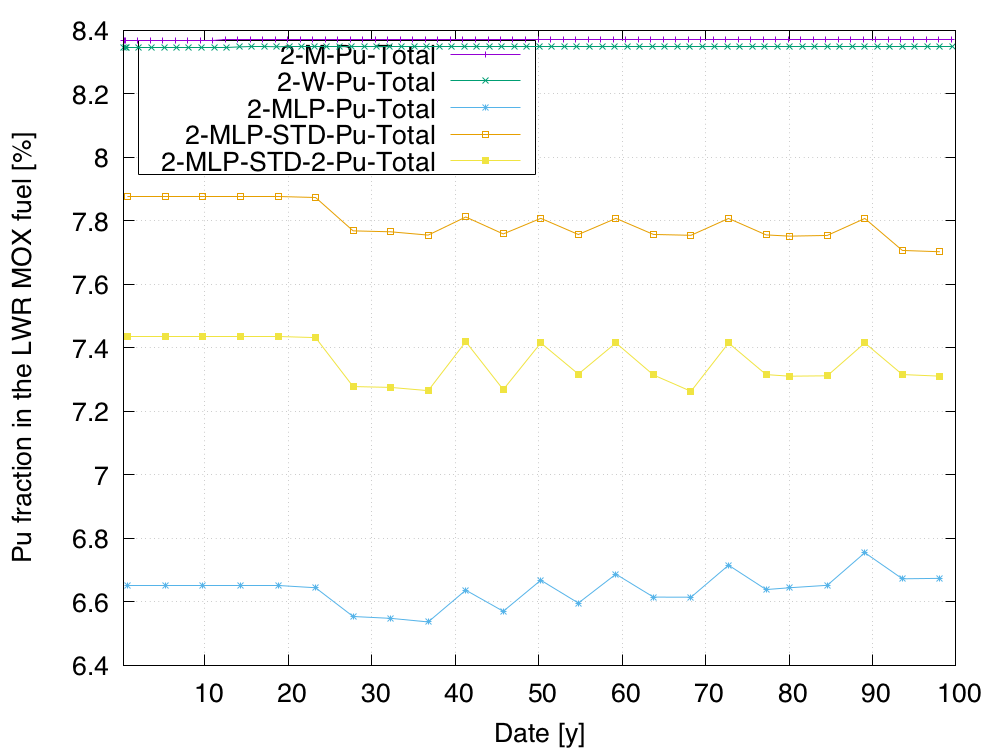
\includegraphics[width=0.7\textwidth]  {img/C_1_2_MOX_pu_contribution}
  \caption{Evolution of the plutonium fraction in the MOX fuel loaded in PWR.
  Those calculation did not include decay process.}
  \label{fig:pufrac_ND}
\end{figure}
%\begin{figure}[h!]
%  \centering
%  
%  \subfigure[Plutonium fraction in the MOX fuel loaded in PWP.\label{fig:pufrac_ND}] 
%    {\epsfig{figure=img/C_1_2_MOX_pu_contribution,width=0.48\textwidth}}
%  \subfigure[Plutonium fraction burned furing the irradiation.\label{fig:puburn_ND}] 
%    {\epsfig{figure=img/C_1_2_MOX_pu_burned,width=0.48\textwidth}}
%  
%  \caption{Evolution of the plutonium loaded in the PWR and burned during the
%    irradiation. Thos calculation are performed  without decay management.\label{fig:pu_nodecay} }
%\end{figure}


On Figure \ref{fig:pufrac_ND}, one can observe the evolution of the plutonium
enrichment loaded in the PWR fuel depending of the model considered for the
fabrication.
The Neural network model using a k∞ of 1.01 clearly under estimate the amount of
plutonium require comparatively to the other models: the require reactivity is
lower. We can observe the effect of the batching (3or 4) on the
neural network models using a k∞ of 1.034, which predict an initial enrichment
close to the one use on the more standard models: $7.5\%$ versus $7.8\%$. Those
models predict a enrichment slightly lower than the one use with the fix mixing
fraction and the Pu-equivalent.
The Pu-equivalent try to mix both stream to reach the composition of the fuel
used in the fixing-fraction method. So it is expected to match it or to be very
close.
For all fabrication model used, the behavior without decay very closed to
expected: we observe a small variation of the amount of plutonium: the
composition of the plutonium is constant with allow the equilibrium to be
maintain. 

%Unstead the recipe based calculation, all the calculation involving Neural
%Network fuel fabrication model, require a dedicated depletion calculation to
%determine the composition of the fuel after irradiation. On Figure
%\ref{fig:puburn_ND}, the evolution of plutonium fraction burned during the
%irradiation for the different models. As expected, all recipe based calculation
%(fix mixing ratio and Pu-equivalent) have very close results around $2.4\%$. The
%only fluctuation here is coming from rounding errors. The Neural network baed
%calculation reach a burning plutonoium amount between $2$ and $2.4\%$.

\subsection{Decay}

\begin{figure}[h!]
  \centering
  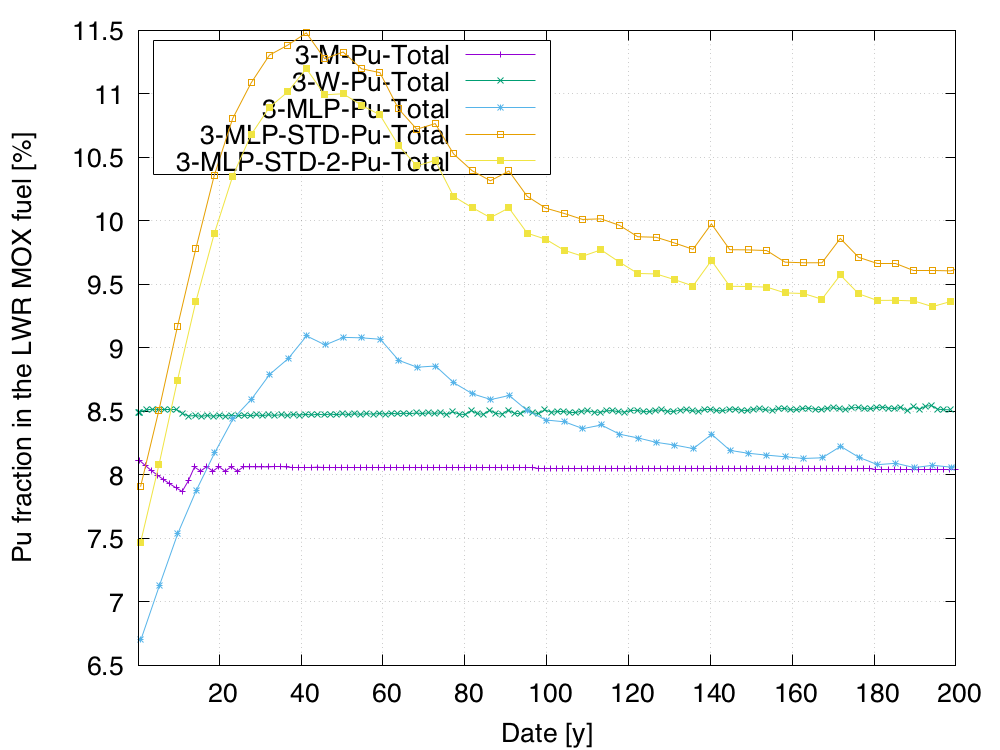
\includegraphics[width=0.7\textwidth]  {img/C_1_3_MOX_pu_contribution}
  \caption{Evolution of the plutonium fraction in the MOX fuel loaded in PWR.
  Those calculation did include decay process.}
  \label{fig:puflow_D}
\end{figure}
%\begin{figure}[h!]
%  \centering
%  
%  \subfigure[Plutonium fraction in the MOX fuel loaded in PWP. \label{fig:pufrac_D}] 
%      {\epsfig{figure=img/C_1_2_MOX_pu_contribution,width=0.48\textwidth}}
%  \subfigure[Plutonium fraction burned furing the irradiation.\label{fig:puburn_D}] 
%      {\epsfig{figure=img/C_1_2_MOX_pu_burned,width=0.48\textwidth}}
%
%  \caption{Evolution of the plutonium loaded in the PWR and burned during the
%    irradiation. Thos calculation are performed  without decay management.\label{fig:pu_decay} }
%\end{figure}

When decay is taking into account, all model base on neural network increase the
enrichment in plutonium by $2.5-3\%$. The $^{241}$Pu decay and change in the
final isotopic composition of the fuel.  The decay of $^{241}$Pu is causing the
degradation of the plutonium quality and to the production of $^{241}$Am (acting
as a neutronics poisons), both of those effect tends to increase the amount of
plutonium require to build the fuel.
The effect of the presence of the initial inventory which is required to start
the calculation, is as limited as possible: all calculation have been tuned to
reduce at the minimum the amount of initial storage (which depends on the model
used).
We can observe (see Figure \ref{fig:puflow_D} and Figure \ref{fig:pu_compo})
that as the $^{241}$Pu fraction decrease and the $^{239}$Pu fraction increase in
the used MOX composition, the amount of plutonium in the fresh fuel reaches an
equilibrium closer to the initial fix ratio.

\begin{figure}[h!]
  \centering
  
  \subfigure[Evolution of the Pu composition in the fresh fuel using the MLP-STD
  fabrication model.\label{fig:pucompo_1}] 
      {\epsfig{figure=img/C_1_3_MLP-STD_MOX_pu_composition,width=0.48\textwidth}}
  \subfigure[Evolution of the Pu composition in the fresh fuel using the
    MLP-STD-2 fabrication model.\label{fig:pu_compo_2}] 
      {\epsfig{figure=img/C_1_3_MLP-STD-2_MOX_pu_composition,width=0.48\textwidth}}

  \caption{ Evolution of the isotopic composition of the plutonium in the fresh MOX fuel.
    \label{fig:pu_compo} } 
  \end{figure}

Even if the different model predictions fail to agree on a common equilibrium,
the point of the study is not determining which calculation is correct or not
(both are probably correct), but to highlight the sensitivity of the equilibrium
state to the isotopic composition and the modeling choice (particularly on
thermal reactor): having too strong constrains on the definition of the fuel
cycle might lead us on the wrong path\dots


In order to support this statement, 3 addition calculations have been performed
using the plutonium equivalent theory. In this calculation the fuel cycle is
the same as the one described as Case 1.3, but the initial inventory has been
increased by a factor 2, 5 and 10.


\section{Plutonium stacking effect}

In the following calculation, the inventory of the J1'' have been increase by a
factor 2, 5, and 10, in order to probe the effect of the of material stacking in
the J1 storage.

\begin{figure}[h!]
  \centering
  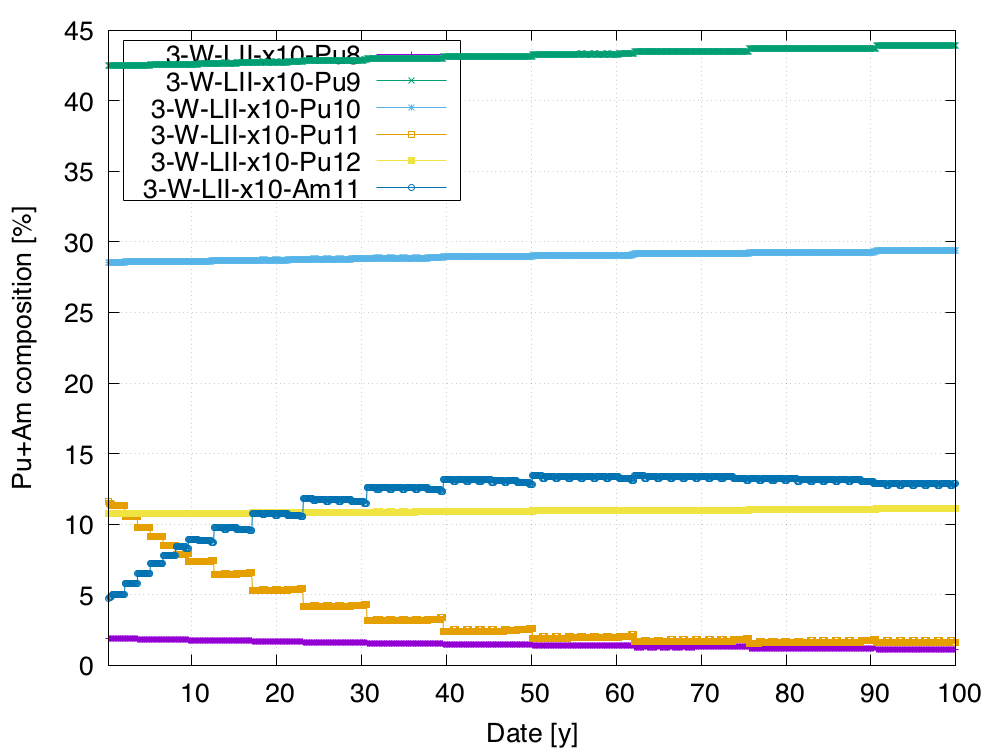
\includegraphics[width=0.6\textwidth]  {img/C_1_3_W_LII_x10_pu_composition}
  \caption{Evolution of the plutonium composition in the J1'' storage in the
  case of the initial inventory has been increased by a factor 10.}
  \label{fig:LII_compo_x10}
\end{figure}

As shown figure \ref{fig:LII_compo_x10}, the fraction of $^{241}$Pu drops from
about $12\%$ to less than $2\%$in about 60y, while the $^{241}$Am rises from
$5\%$ to about $12\%$. To illustrate this effect one only show the configuration
with the strongest. $^{241}$Pu and $^{241}$Am finds a respective equilibrium
around $11\%$ and $1\%$ for the normal calculation, $10\%$ and $2\%$ in the
''x2'' calculation and, $3\%$ and $10\%$ in the ''x5'' case. This conversion of
the $^{241}$Pu into $^{241}$Am induce an increased average time the separate
plutonium spend in storage before being used to build fresh MOX fuel.

\begin{figure}[h!]
  \centering
  
  \subfigure[J1'' stream flow.\label{fig:E1_LII}] 
      {\epsfig{figure=img/C_1_3_W_LII_J1s.png,width=0.48\textwidth}}
  \subfigure[E3'' stream flow.\label{fig:E3_LII}] 
      {\epsfig{figure=img/C_1_3_W_LII_E3s.png,width=0.48\textwidth}}

  \caption{ Evolution of the J1'' and E3'' stream flow accordingly to the size
    of initial inventory. \label{fig:LII} } 
  \end{figure}

As observed on Figure \ref{fig:LII}, the decay of the $^{241}$Pu has a direct
impact on the different contribution of E3'' and J1'' stream. The model trying
to balance the loss of reactivity of the J1'' stream by increasing the amount of
E3'' stream in the mix. The variation can be up to $10\%$ in the worse case
after 100y.

\section{Discussion}

In conclusion, this study has show the impact of different way to model
the MOX fuel fabrication considering decay or not.
The Pu-equivalence theory reach an equilibrium (in the mixing ratio of E3'' and
J1'' stream) very close to the fix mixing ratio, when the decay is not activate.
This was expected: the Pu-equivalent model try to build a MOX fuel with the same
initial reactivity as the one used in the fix mixing ratio calculation, so it
used the same mixing ratio\dots  

Nevertheless we can observe a variation of $20\%$ when taking into account the
decay process in the contribution of E3'' and J1'' stream. This variation is a
direct consequence of the decay of $^{241}$Pu producing $^{241}$Am, which
decrease the reactivity potential of J1'' ( loss of the $^{241}$Pu reactivity
and neutronic poisoning of the $^{241}$Am). The E3'' reactivity barely changes:
the $^{241}$Pu is negligible in E3'' composition.

The main difference, between calculation using the CLASS model and the other
calculation, is the recalculation of the fuel evolution during irradiation. 

The calculation using the CLASS model based on neural network support those this
observation. Without decay, those model predict a constant plutonium enrichment
in the MOX fuel $6.6\%$, $7.4\%$ and $7.8\%$ depending on the model used versus
about $8.4\%$ for the mixing ratio. This disagreement of few percents in the
plutonium enrichment, is directly a consequence of the modeling differences
between the models.  But this common flat behavior highlight that the steady
state is well described by all simulation when the decay are not considered
Even if the CLASS model did not exactly agree on the plutonium enrichment
require in the fuel to get the correct reactivity properties, because the
equilibrium did not change, the output composition recalculated by the CLASS
model if very close the out recipe used by the other calculation.

When considering the decay, all the CLASS model need about 180y to reach a
proper equilibrium. This is because the composition of the plutonium
strongly impact its enrichment in the fresh fuel (as shown in the Pu-equivalent
case). And the fresh fuel composition will strongly impact the plutonium
composition at the end of irradiation. 

Moreover, the last part of the study, shows the impact of the stacked plutonium
on its composition and then on the fuel fabrication. Those kind of material
stacking could the consequences of disruption if the material flow of in a real
cycle. Having very strong constrains might lead to ignore such disruption
effect. In order to mimic a potential material stacking, the same steady state
calculation have been perform three times increasing the amount of initial
inventory require to start the calculation by a factor 2, 5 and 10. In all
cases, $^{241}$Pu stacking induce $^{241}$Am production which impact strongly
the mixing ration between E3'' and J1'' ( $5\%$ to $10\%$), which might have a
strong effect on the used fuel composition, specially with thermal reactor, were
the different cross section are so sensitive to the composition of the fuel.



%----------------------------------------------------------------------------------------
%        BIBLIOGRAPHY
%----------------------------------------------------------------------------------------

\bibliographystyle{unsrt}

\bibliography{bib}

%----------------------------------------------------------------------------------------

\end{document}

